\documentclass[a4paper]{article}
\usepackage[margin=0.5in]{geometry}
\usepackage{xcolor}
%\usepackage[dvipdfm]{graphicx}
\usepackage{graphicx}

\newcommand{\brown}{\color{brown}}

\newenvironment{codesnip}[1]
{\begin{tightcenter}\begin{minipage}{.85\textwidth}#1}
{\end{minipage}\end{tighcenter}}


\title{Model Documentation}
\author{Luis Suazo}
\date{}

\begin{document}
\maketitle

\section{Background}	
\begin{itemize}
  \item Competition Name: Predict Future Sales
  \item Team Name: None
  \item Private Leaderboard Score: TBA
  \item Private Leaderboard Place: TBA
  \item Name: Luis Suazo
  \item Location: USA
  \item Email: None
  \item Academic Background: PhD in Theoretical Physics
  \item Professional Background: Systematic Trader
  \item Prior Experience: Some Data Science Education
  \item Time Spent on Competition: Somewhere around 20 hours
\end{itemize}	

\section{Summary}
The main model that I use is a gradient boosting machine, namely the xgboost implementation. I also use a much simpler elastic net model with fewer and simpler features, whose prediction is passed to the main xgb model - that is, the models are stacked. As far as features, I aggregated the raw data into monthly data, since that is what we are trying to predict. For the simple linear model, I use lagged values of sales, and shop/item aggregation of sales. For the xgb model I create many features to capture item, shop, and temporal information. Furthermore I create rolling satistics or exponentially weighted statistics for most of these features to incorporate past behavior. Finaly, I stack twelve months of data (including the lagged features) to train a model. I use a rolling, causal cross validation strategy to test my model fully out of sample, with each new month. The most important features, other than the exponentially weighted mean of monthly sales, are mean encodings for shops, items, items category, and a shop-item cat interaction feature. My model takes about 12 minutes to train, and it takes about 20 minutes to process the data (including fitting a simpler linear model).

\section{Feature Selection/Engineering}

The most important features for my model were target encoding of categorical variables, and even interactions between categorical variables. Namely target encoding each item and each shop, using both nubmer of sales and total income (sales * price). The interaciton that seemed most important was the shop-category interaction. This is not surprising given that some shops focus on some items/item categories. So it was useful to capture this relationship.
Target encoding this variable led to a very important feature. Another important feature was the prediction from the linear model used in stacking. And almost as important were features derived from a k-means clustering of the shops withe respect to the total sales of items in each category. From these clusters, I derived several statistics that I then lagged, and used as features.

My feature selection process was simply dropping features that ended up with little importance in the trained xgboost models. I did not create a vast amount of features, as I was very targeted in the feature generation process. So I eneded up keeping most of the features I created, since they seemed to provide some use to the model.


\begin{center}
  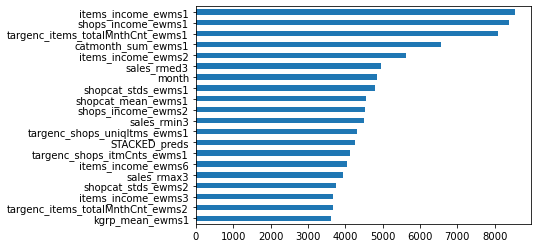
\includegraphics[width=15cm]{Top20.png}
\end{center}

\section{Training Methods}

Once I created all the features for each month of data (including lagged features), I simply stacked several months of data together and use this to train the model. This seemed to work relatively well. I did try creating a linear model, with lagged raw features, to use in ensembling. However, it seemse to always bring down the predictive power, no matter what weighted average I used. So instead, I ended up using that model as another feature in the main model - that is, I stacked them.

\section{Interesting Findings}

I believe the most important trick I used was target encoding, with k means being a close second. Though I expect most other participants used these tricks too. I created several time based features, like holidays, weekdays, weekends, etc, but they were not used much by the model. I suspect this is an area that proably needs some more refined tricks, because there is clearly a strong temporal behavior. It also bears mentioning that clipping the final prediction was crucial.

\section{Simple Features And Methods}

A model based solely on exponentially weighted moving average of sales, and target encoding of shops, items, item category, and shop-category interaction goes a long ways. Even with a reduced strength xgb, like 100 trees and max depth 10, this model performs almost a good as my best model.

\section{Model Execution Time}

Training the final model takes about 20 minutes. To perform the full rolling cross validation takes about 3 hours. Once trained, the predictions are obtained in less than a minute. The simplified model can be trained in about 5 minutes, and can create predictions in less than a minute.


\end{document}
